% !TeX root = ../../main.tex
\section{Architecture}\label{section:architecture}

The experiments presented in the next section are implemented as part of the \gls{UBII} front end\footnote{Applications are often separated into a front end and a back end. The front end displays information to the users, while the back end processes the logic.}. The same applies to the smart device client, as illustrated in Figure~\ref{fig:architecture}. Both applications run in a web browser and communicate with the \gls{UBII} server\footnote{Figure~\ref{fig:architecture} illustrates no direct connection between the smartphone or \gls{PC} and the \gls{UBII} server for the sake of simplicity. However, when running the software, a connection is established, since the \gls{UBII} front end runs on the client device.}. The smart device client runs on a smartphone. In most scenarios, the smartphone is connected to the server using \gls{WLAN}.

\begin{figure}[H]
  \centering
  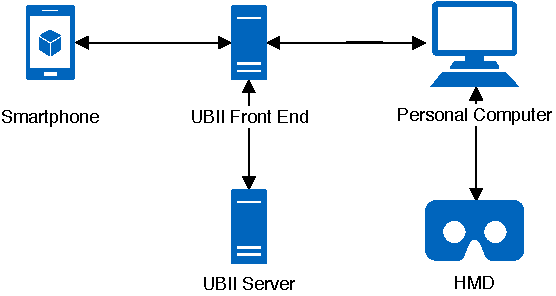
\includegraphics[width=10cm]{figures/implementation/architecture.pdf}
  \caption[System architecture]{This diagram shows the simplified architecture of the complete system. An arrow means that the connected applications exchange data. Multiple instances of the smartphone or front end are combined into one diagram entity. The web server, serving the front end, is hidden for the sake of simplicity.}\label{fig:architecture}
\end{figure}

A \gls{PC} running the \gls{HMD} driver software and a web browser with the experiments running in Three.js is used as a bridge between the \gls{HMD} and the \gls{UBII} front end. This setup may vary depending on the \gls{VR} headset. The Google Cardboard, for example, does not require any \gls{PC} in between.

